\section{Data annotation application}\label{sec:data_annotation_application}

This is a simple web-application which provides a user interface for users to label the crawled pages.
On load, it will present a randomly selected page from the crawled set of pages, and the user can first classify it as a product page, product list page, error page, or other.
If the page is classified as a product page, the user can then annotate the relevant product information, including the product title, image, price, brand, and stock status.

Figure~\ref{fig:labeller} shows a screenshot of the data annotation application, which is designed to be simple and intuitive to use, allowing users to quickly and accurately label the crawled pages.
The application shows two side-by-side views of the page, with the first being the original page and the second being a minimized view of the page, which is generated by the HTML minimizer module.
On the right side of the page, there are a set of input fields for the user to enter the relevant product information, and a set of buttons to classify the page and submit the annotations.
Once submitted, the annotated data will be stored in the \texttt{page\_labels} table in the database, along with the HTML content of the corresponding page.
The annotated data will be used to train the page classifier and information extractor modules, which will enable the system to automatically classify and extract relevant product information from the crawled pages.

\begin{figure}[h]
    \centering
    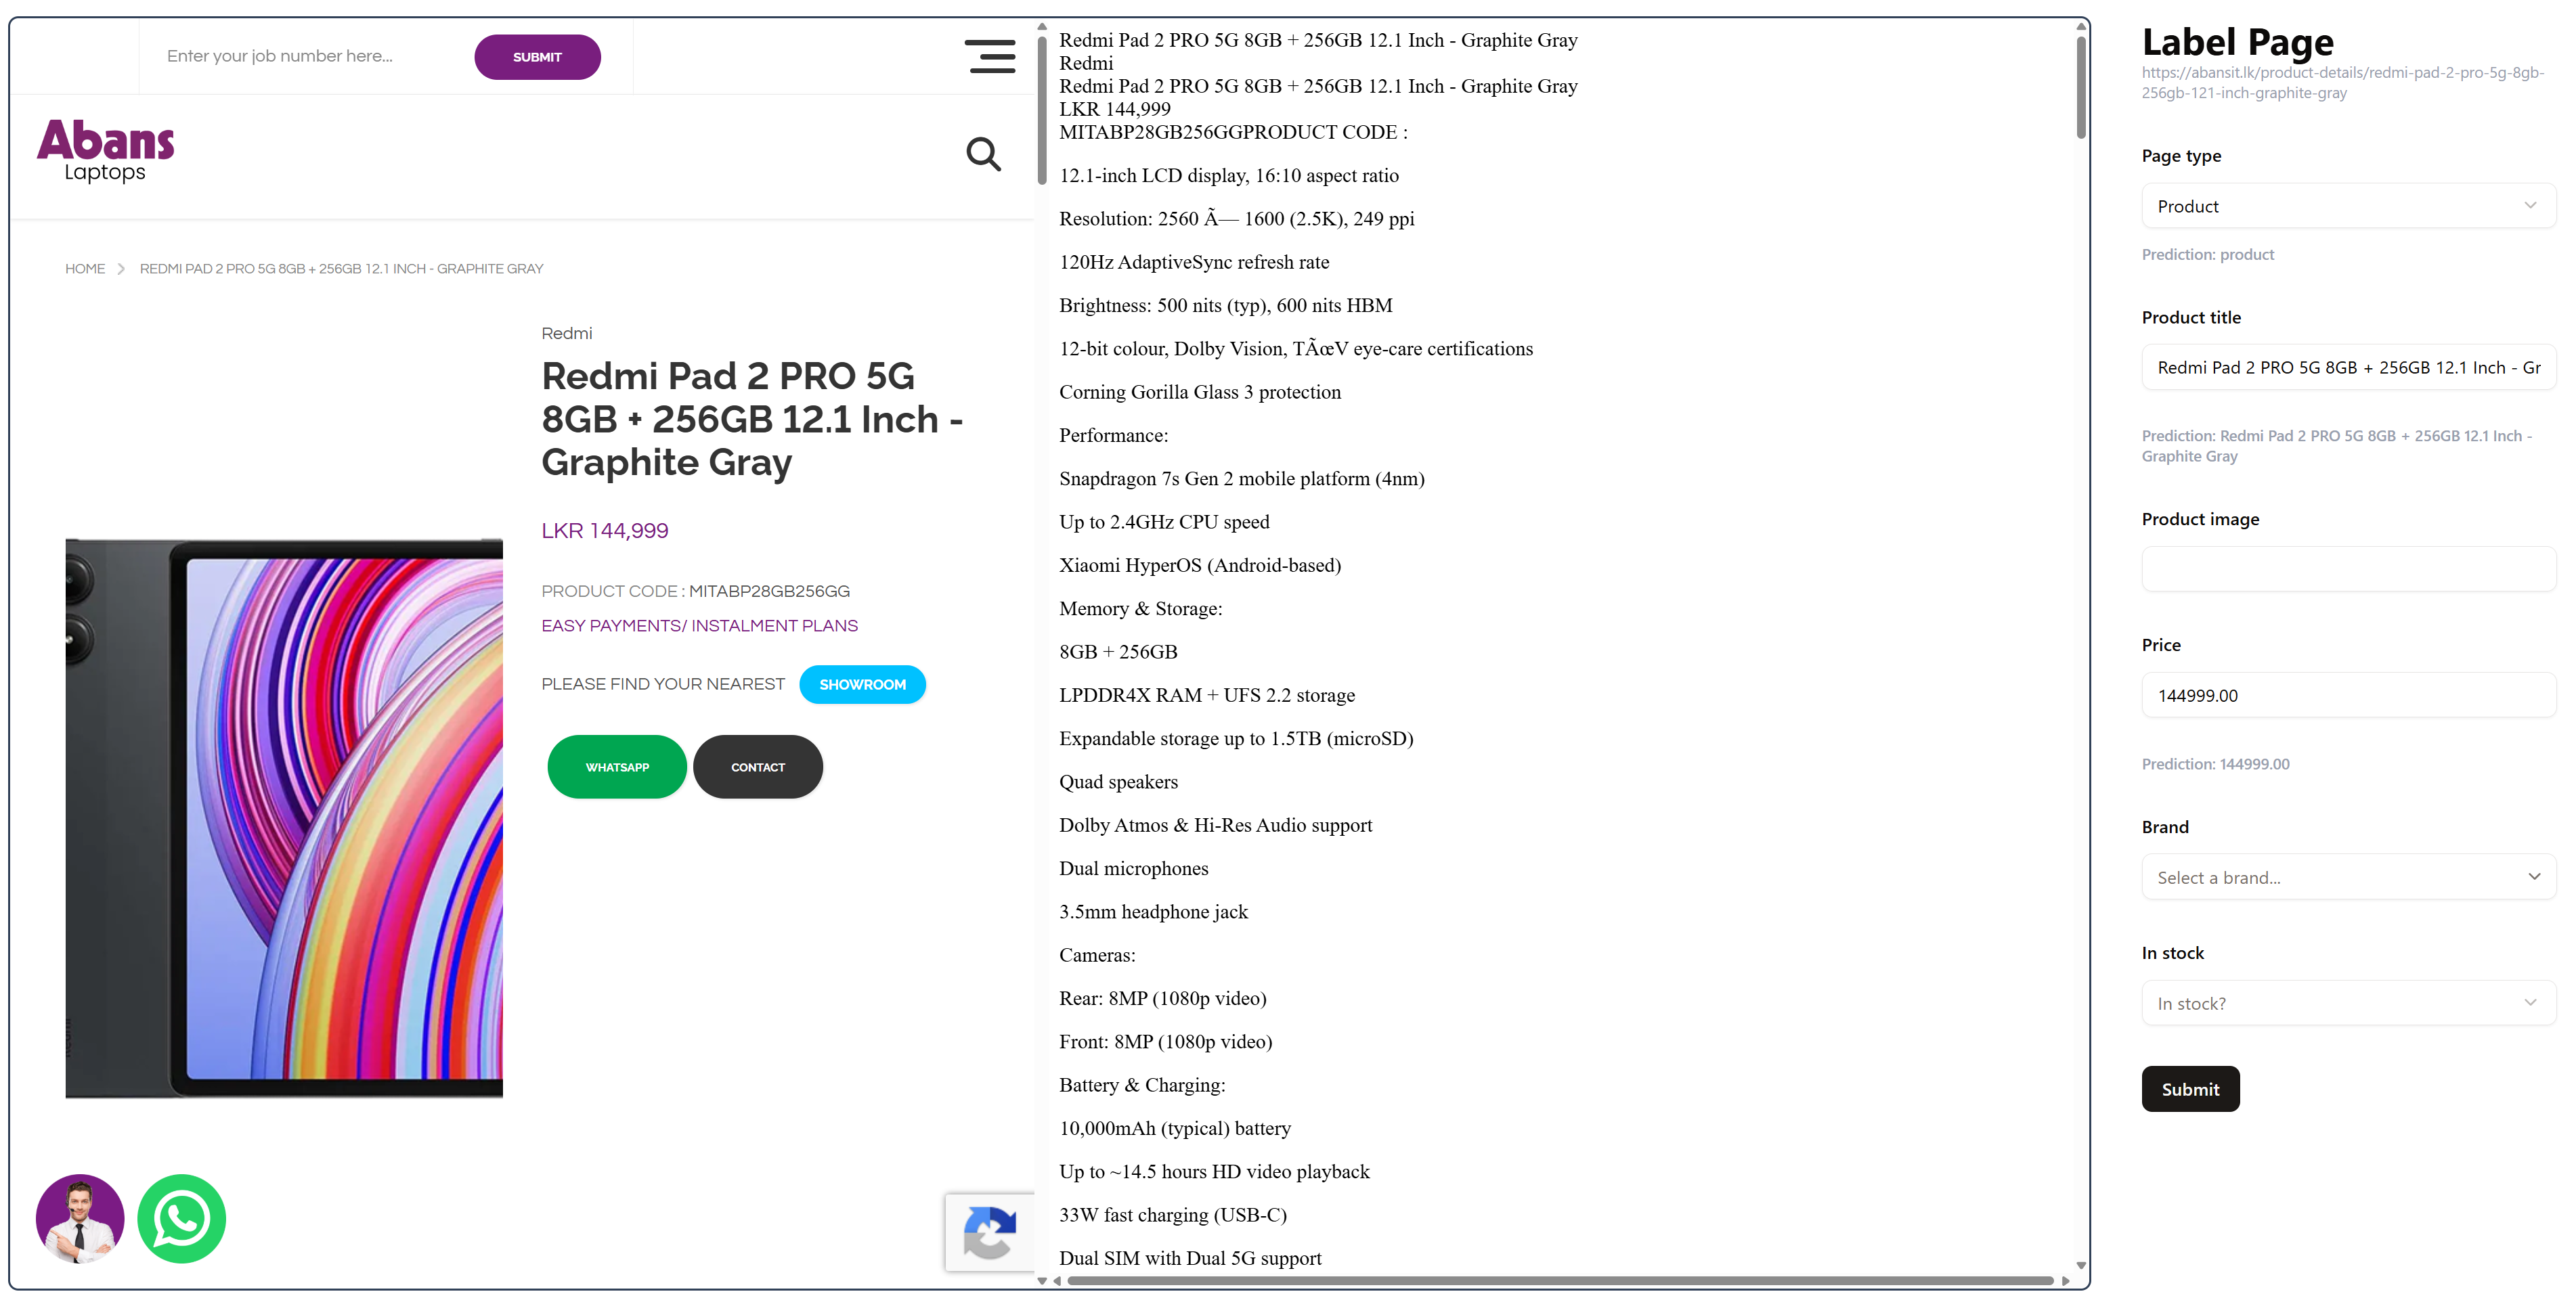
\includegraphics[width=0.8\textwidth]{images/labeller_screenshot}
    \caption{Screenshot of the data annotation application.}
    \label{fig:labeller}
\end{figure}

This application is developed with Next.js, a React framework for building server-side rendered web applications.
Next.js was selected for this task as it allows for the quick development of simple, uncomplex web applications, and provides a good developer experience.